% Options for packages loaded elsewhere
\PassOptionsToPackage{unicode}{hyperref}
\PassOptionsToPackage{hyphens}{url}
%
\documentclass[
]{article}
\usepackage{lmodern}
\usepackage{amssymb,amsmath}
\usepackage{ifxetex,ifluatex}
\ifnum 0\ifxetex 1\fi\ifluatex 1\fi=0 % if pdftex
  \usepackage[T1]{fontenc}
  \usepackage[utf8]{inputenc}
  \usepackage{textcomp} % provide euro and other symbols
\else % if luatex or xetex
  \usepackage{unicode-math}
  \defaultfontfeatures{Scale=MatchLowercase}
  \defaultfontfeatures[\rmfamily]{Ligatures=TeX,Scale=1}
\fi
% Use upquote if available, for straight quotes in verbatim environments
\IfFileExists{upquote.sty}{\usepackage{upquote}}{}
\IfFileExists{microtype.sty}{% use microtype if available
  \usepackage[]{microtype}
  \UseMicrotypeSet[protrusion]{basicmath} % disable protrusion for tt fonts
}{}
\makeatletter
\@ifundefined{KOMAClassName}{% if non-KOMA class
  \IfFileExists{parskip.sty}{%
    \usepackage{parskip}
  }{% else
    \setlength{\parindent}{0pt}
    \setlength{\parskip}{6pt plus 2pt minus 1pt}}
}{% if KOMA class
  \KOMAoptions{parskip=half}}
\makeatother
\usepackage{xcolor}
\IfFileExists{xurl.sty}{\usepackage{xurl}}{} % add URL line breaks if available
\IfFileExists{bookmark.sty}{\usepackage{bookmark}}{\usepackage{hyperref}}
\hypersetup{
  pdftitle={main},
  pdfauthor={Dexter Weighell},
  hidelinks,
  pdfcreator={LaTeX via pandoc}}
\urlstyle{same} % disable monospaced font for URLs
\usepackage[margin=1in]{geometry}
\usepackage{longtable,booktabs}
% Correct order of tables after \paragraph or \subparagraph
\usepackage{etoolbox}
\makeatletter
\patchcmd\longtable{\par}{\if@noskipsec\mbox{}\fi\par}{}{}
\makeatother
% Allow footnotes in longtable head/foot
\IfFileExists{footnotehyper.sty}{\usepackage{footnotehyper}}{\usepackage{footnote}}
\makesavenoteenv{longtable}
\usepackage{graphicx,grffile}
\makeatletter
\def\maxwidth{\ifdim\Gin@nat@width>\linewidth\linewidth\else\Gin@nat@width\fi}
\def\maxheight{\ifdim\Gin@nat@height>\textheight\textheight\else\Gin@nat@height\fi}
\makeatother
% Scale images if necessary, so that they will not overflow the page
% margins by default, and it is still possible to overwrite the defaults
% using explicit options in \includegraphics[width, height, ...]{}
\setkeys{Gin}{width=\maxwidth,height=\maxheight,keepaspectratio}
% Set default figure placement to htbp
\makeatletter
\def\fps@figure{htbp}
\makeatother
\setlength{\emergencystretch}{3em} % prevent overfull lines
\providecommand{\tightlist}{%
  \setlength{\itemsep}{0pt}\setlength{\parskip}{0pt}}
\setcounter{secnumdepth}{5}

\title{main}
\author{Dexter Weighell}
\date{}

\begin{document}
\maketitle

{
\setcounter{tocdepth}{2}
\tableofcontents
}
\hypertarget{introduction}{%
\subsection{\texorpdfstring{\textbf{Introduction}}{Introduction}}\label{introduction}}

Egg egg egg, egg egg egg (Hinde 1958). As seen in figure \includegraphics{figures/egg-figures.jpg}

\hypertarget{methods}{%
\subsection{\texorpdfstring{\textbf{Methods}}{Methods}}\label{methods}}

\hypertarget{results}{%
\subsection{\texorpdfstring{\textbf{Results}}{Results}}\label{results}}

chaffinches have a greater mean mass

\begin{verbatim}
## 
##  Shapiro-Wilk normality test
## 
## data:  chaff2$mass
## W = 0.98873, p-value = 0.9555
\end{verbatim}

\begin{verbatim}
## 
## Call:
## lm(formula = mass ~ sex, data = chaff2)
## 
## Coefficients:
## (Intercept)     sexmales  
##      20.480        1.795
\end{verbatim}

\begin{verbatim}
## 
## Call:
## lm(formula = mass ~ sex, data = chaff2)
## 
## Residuals:
##     Min      1Q  Median      3Q     Max 
## -5.2750 -1.7000 -0.3775  1.6200  4.1250 
## 
## Coefficients:
##             Estimate Std. Error t value Pr(>|t|)    
## (Intercept)  20.4800     0.4795  42.712   <2e-16 ***
## sexmales      1.7950     0.6781   2.647   0.0118 *  
## ---
## Signif. codes:  0 '***' 0.001 '**' 0.01 '*' 0.05 '.' 0.1 ' ' 1
## 
## Residual standard error: 2.144 on 38 degrees of freedom
## Multiple R-squared:  0.1557, Adjusted R-squared:  0.1335 
## F-statistic: 7.007 on 1 and 38 DF,  p-value: 0.01175
\end{verbatim}

\includegraphics[width=468px]{markdown_files/figure-latex/import data analysis-1}

\begin{figure}
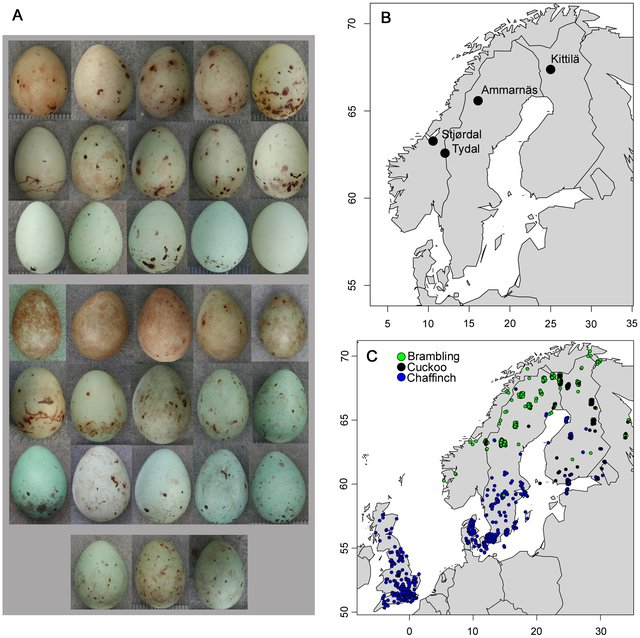
\includegraphics[width=0.3\linewidth]{figures/egg-figure} \caption{egg}\label{fig:egg-figure}
\end{figure}

\hypertarget{discussion}{%
\subsection*{\texorpdfstring{\textbf{Discussion}}{Discussion}}\label{discussion}}
\addcontentsline{toc}{subsection}{\textbf{Discussion}}

\hypertarget{refs}{}
\leavevmode\hypertarget{ref-Hinde}{}%
Hinde, R. A. 1958. ``Alternative Motor Patterns in Chaffinch Song.'' \emph{Animal Behaviour} 6 (3): 211--18. \url{https://doi.org/https://doi.org/10.1016/0003-3472(58)90053-8}.

\end{document}
